\documentclass{beamer}
\usepackage{listings}
\lstset{
%language=C,
frame=single, 
breaklines=true,
columns=fullflexible
}
\usepackage{subcaption}
\usepackage{url}
\usepackage{tikz}
\usepackage{graphicx}
\usepackage{tkz-euclide} % loads  TikZ and tkz-base
%\usetkzobj{all}
\usetikzlibrary{calc,math}
\usepackage{float}
\usepackage{amsthm}
\newcommand\norm[1]{\left\lVert#1\right\rVert}
\renewcommand{\vec}[1]{\mathbf{#1}}
\newcommand{\R}{\mathbb{R}}
\newcommand{\C}{\mathbb{C}}
\newcommand{\comb}[2]{{}^{#1}\mathrm{C}_{#2}}
\providecommand{\brak}[1]{\ensuremath{\left(#1\right)}}
\providecommand{\abs}[1]{\vert#1\vert}
\providecommand{\fourier}{\overset{\mathcal{F}}{ \rightleftharpoons}}
\providecommand{\sbrak}[1]{\ensuremath{{}\left[#1\right]}}
\usepackage[export]{adjustbox}
\usepackage[utf8]{inputenc}
\usepackage{amsmath}
\usepackage[version=4]{mhchem}
\usetheme{Boadilla}
\title{Convergence}
\author{Vikhyath Sai Kothamasu}
\institute{IITH}
\date{\today}
\begin{document}

\begin{frame}
\titlepage
\end{frame}
\begin{frame}{Question}
\begin{block}{GATE 2018 (MA), Q. 25 (Pg.7)}
Let $\{X_j\}$ be a sequence of independent Bernoulli random variables with $\mathbb{P}(X_j=1) = \frac{1}{4}$ and let $Y_n = \frac{1}{n} \sum_{j=1}^{n}X_j^2$. Then $Y_n$ converges, in probability, to $\rule{2cm}{0.15mm}$ .
\end{block}
\end{frame}
\begin{frame}{Various Convergences}
%\frametitle{Various Convergences}
In probability theory, there exist several different notions of convergence of random variables.
\begin{enumerate}
    \item Convergence in distribution or Converge weakly 
        \begin{align}
            \lim_{n\rightarrow\infty}F_{X_n}(x) = F_X(x) \quad \forall x \in \mathbb{R}
        \end{align}
    \item Convergence in probability
        \begin{align}
            \lim_{n\rightarrow\infty} \Pr{(\abs{X_n-X} \geq \epsilon)} = 0
        \end{align}
    \item Almost sure convergence
        \begin{align}
            \Pr{(\lim_{n\rightarrow\infty}X_n=X)} = 1
        \end{align}
\end{enumerate}
\end{frame}
\begin{frame}{More convergences}
\begin{enumerate}
  \setcounter{enumi}{3}
  \item Sure convergence or pointwise convergence
    \begin{align}
        \lim_{n\rightarrow\infty} X_n(\omega) = X(\omega) \quad \forall \omega \in \Omega
    \end{align}
    where $\Omega$ is the sample space of the underlying probability space over which the random variables are defined.
    \item Convergence in mean. Given a real number $r\geq 1$
        \begin{align}
            \lim_{n\rightarrow\infty}E(\abs{X_n-X}^r) = 0 \quad 
        \end{align}
\end{enumerate}
\end{frame}
\begin{frame}{Properties}
There are several properties involving different types of convergence of which few are listed below
\begin{enumerate}
    \item Almost sure convergence implies convergence in probability
    \item Convergence in probability implies convergence in distribution
    \item If $X_n$ converges in distribution to a constant c, then $X_n$ converges in probability to c
    \item Convergence in r-th order mean implies convergence in lower order mean, assuming that both orders are greater than or equal to one
    \item Convergence in the r-th mean, for $r\geq1$, implies convergence in probability \label{property 5}
\end{enumerate}
For more properties, refer to the properties section in https://en.wikipedia.org/wiki/Convergence\_of\_random\_variables
\end{frame}

\begin{frame}{Proof of property \eqref{property 5}}
\begin{block}{Proof}
\begin{align}
    \text{For any }\epsilon > 0, \quad &
    \\\Pr{(\abs{Y_n-Y}\geq \epsilon)} &= \Pr{(\abs{Y_n-Y}^2\geq \epsilon^2)}
    \\\Pr{(\abs{Y_n-Y}\geq \epsilon)}  &\leq \frac{E\abs{Y_n-Y}^2}{\epsilon^2} 
    \text{ (by Markov's Inequality)}
    \\\lim_{n\rightarrow \infty} E(\abs{Y_n-Y}^2) &= 0 
    \\0 \leq  \lim_{n\rightarrow \infty}\Pr{(\abs{Y_n-Y}\geq \epsilon)}  &\leq \frac{0}{\epsilon^2}
    \\   \lim_{n\rightarrow \infty}\Pr{(\abs{Y_n-Y}\geq \epsilon)} &= 0 \quad \forall \epsilon >0
\end{align}
\end{block}
\end{frame}
\begin{frame}{Markov's Inequality}
If $X$ is a non-negative random variable and $a>0$, then the probability that $X$ is at least $a$ is at most the expectation of $X$ divided by $a$:
\begin{align}
    \Pr{(X\geq a)} \leq \frac{E(X)}{a}
\end{align}
    
\end{frame}

\begin{frame}{Solution}
\begin{align}
    \Pr{(X_j=1)} &= \frac{1}{4}
    \\\Pr{(X_j=0)} &= 1 - \frac{1}{4} = \frac{3}{4}
    \\Y_n &= \frac{1}{n} \sum_{j=1}^{n}X_j^2 
    \\&= \frac{1}{n} \sum_{j=1}^{n}X_j
    \\\Pr{(Y_n = y)} &= \comb{n}{ny} \brak{\frac{1}{4}}^{ny} \brak{\frac{3}{4}}^{n-ny}
    \\\Pr{(Y_n = \frac{k}{n})} &= \comb{n}{k} \brak{\frac{1}{4}}^{k} \brak{\frac{3}{4}}^{n-k}
\end{align}
\end{frame}
\begin{frame}{Solution contd.}
\begin{align}
    E\brak{\abs{Y_n-\frac{1}{4}}^2} &= E\brak{Y_n^2 - \frac{1}{2}Y_n + \frac{1}{16}}
    \\&= E(Y_n^2) - \frac{1}{2}E(Y_n) + \frac{1}{16} \label{equation 0}
    \\E(Y_n^2) &= \sum_{k=0}^n\brak{\frac{k}{n}}^2\Pr{\brak{Y_n=\frac{k}{n}}}
    \\&= \sum_{k=0}^{n} \brak{\frac{k^2}{n^2}}\comb{n}{k} \brak{\frac{1}{4}}^{k} \brak{\frac{3}{4}}^{n-k}
    \\&=  \frac{1}{16} + \frac{3}{16n} \label{equation 2}
\end{align}
\end{frame}
\begin{frame}{Solution contd.}
\begin{align}
    E(Y_n) &= \sum_{k=0}^n\frac{k}{n}\Pr{\brak{Y_n=\frac{k}{n}}}
    \\&= \sum_{k=0}^{n} \brak{\frac{k}{n}}\comb{n}{k} \brak{\frac{1}{4}}^{k} \brak{\frac{3}{4}}^{n-k}
    \\&= \frac{1}{4} \label{equation 3}
\end{align}
Using equation \eqref{equation 2},
\begin{align}
    E\brak{\abs{Y_n-\frac{1}{4}}^2} &= \frac{1}{16}+ \frac{3}{16n}-\frac{1}{2}\times\frac{1}{4} + \frac{1}{16}
    \\&= \frac{3}{16n}
\end{align}
\end{frame}
\begin{frame}{Solution contd.}
 \begin{align}
    \lim_{n\rightarrow \infty} E\brak{\abs{Y_n-\frac{1}{4}}^2} &=  \lim_{n\rightarrow \infty}  \frac{3}{16n}
    \\&= \frac{3}{16}\lim_{n\rightarrow \infty}\frac{1}{n}
    \\&= 0
\end{align}
Thus, $Y_n$ converges, in mean square, to $\frac{1}{4}$ and hence $Y_n$ converges, in probability, to $\frac{1}{4}$.
\end{frame}
\begin{frame}{Figures}
\begin{figure}[!ht]
\centering
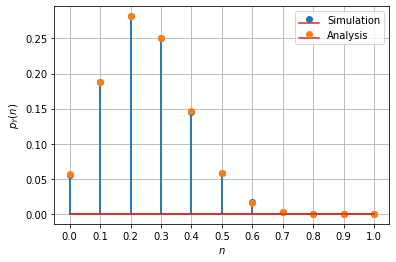
\includegraphics[width=0.8\columnwidth]{pmf.png}
\caption{The PMF distribution of $Y_n$ for n=10}
\label{rect}
\end{figure}
\end{frame}
\begin{frame}{Figures}
\begin{figure}[!ht]
\centering
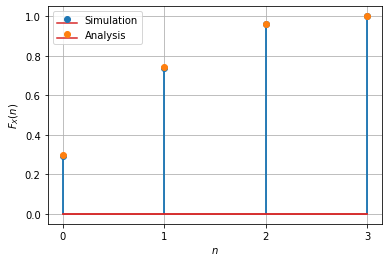
\includegraphics[width=0.8\columnwidth]{cdf.png}
\caption{The CDF distribution of $Y_n$ for n=10}
\label{rect}
\end{figure}
\end{frame}
\end{document}